\chapter{Metodologia}
\label{chapter:Metodologia}

A partir das pesquisas realizadas e documentadas no Apêndice \nameref{apend_chap:metodologia}, pôde-se definir a metodologia aplicada ao trabalho. Este trabalho possui metodologias específicas para a realização do levantamento bibliográfico bem como para estabelecer como proceder nas atividades de desenvolvimento.

A seguir serão apresentadas as duas metodologias e como estas foram aplicadas ao longo deste trabalho.

\section{Metodologia de Pesquisa}

Analisando-se o tema proposto para este trabalho, é possível perceber que se trata de uma pesquisa aplicada \cite{Silva:Tafner:2007}, uma vez que todo levantamento bibliográfico visa a compreensão dos temas, sendo esses conhecimentos adquiridos aplicados no desenvolvimento.

A abordagem é tanto quantitativa quanto qualitativa.

Com relação aos objetivos da pesquisa, considera-se que é uma pesquisa exploratória \cite{Gil:2010}, devido à necessidade encontrada em entender adequadamente o problema apresentado e se obter um maior entendimento de todos os temas relacionados ao que se propõe.

No contexto dos procedimentos técnicos, foi aplicada a pesquisa bibliográfica \cite{Silva:Tafner:2007}, visando o levantamento de fontes para se alcançar o conhecimento necessário para a realização do trabalho.

Por fim, no intuito de analisar os resultados obtidos no projeto, utilizou-se a pesquisa-ação \cite{Silva:Tafner:2007}. Nesse caso, foram conduzidos ciclos evolutivos visando:

\begin{enumerate}
	\item A identificação de não conformidades;
	\item A execução de ações estratégicas no intuito de melhorar essas não conformidades;
	\item A análise dos resultados obtidos com a aplicação dessas ações.
\end{enumerate}

\section{Metodologia de Desenvolvimento}

A metodologia de desenvolvimento seguiu algumas práticas ágeis já consolidadas. Basicamente, utilizou-se as práticas ágeis propostas na metodologia \textit{Scrum}\footnote{\url{http://www.desenvolvimentoagil.com.br/scrum/}}, como o uso de histórias de usuários, reuniões diárias (no contexto do trabalho foram de dois em dois dias), \textit{sprints} de quinze dias, \textit{backlog do produto} e \textit{backlog de sprint}. Quando necessário, voltou-se também à algumas práticas do \textit{XP}\footnote{\url{http://www.desenvolvimentoagil.com.br/xp/}}, como o uso de integração contínua, pareamento e \textit{planning poker} para estimativa de pontos das histórias.

\section{Fluxo de Trabalho}

A Figura \ref{processo tcc} apresenta o fluxo de trabalho que orientou a condução desse projeto.

\begin{figure}[h]
	\centering
	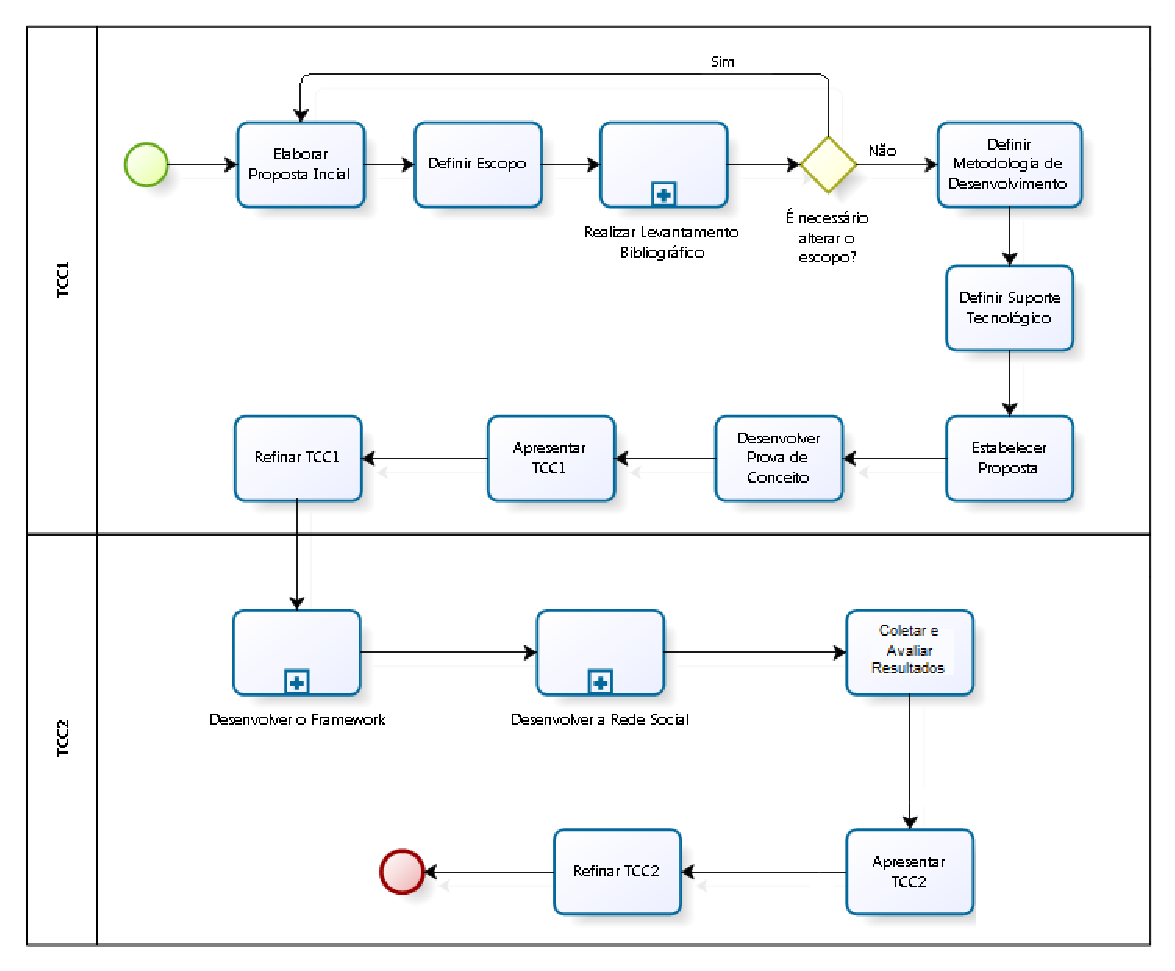
\includegraphics[scale=0.6]{figuras/capitulo4/processo_tcc.eps}
	\caption{Fluxo de trabalho}
	\label{processo tcc}
\end{figure}

Primeiramente, a ideia inicial para o projeto foi definida bem como trabalhada, obtendo como resultado a proposta (em seu esboço preliminar). A partir dessa proposta, o escopo inicial foi definido, conferindo base para a realização do levantamento bibliográfico. Ao final, voltou-se o fluxo ao início, visando um melhor refinamento do que já havia sido realizado.

A partir da proposta inicial, foram definidos a metodologia de desenvolvimento, o suporte tecnológico e uma proposta mais concreta, a qual foi de fato desenvolvida ao longo do TCC. Para comprovar a viabilidade da proposta, uma prova de conceito foi elaborada.

Por fim, o trabalho foi apresentado e refinado de acordo com as observações da banca examinadora.

A segunda parte do fluxo apresenta as atividades relacionadas ao desenvolvimento do \textit{framework} e da rede social que exemplificou o uso deste \textit{framework}, comprovando assim a sua instanciação e aplicabilidade. Na última etapa, os resultados obtidos foram coletados e o trabalho final foi apresentado e refinado.

Como pode ser visto no processo apresentado na Figura \ref{processo tcc}, existem duas etapas  envolvendo desenvolvimento, no caso: ``Desenvolver o \textit{Framework}'' e ``Desenvolver a Rede Social''. Cada uma dessas etapas, seguiu um Processo alternativo, como mostrado na Figura \ref{Processo desenvolvimento}.

\begin{figure}[h]
	\centering
	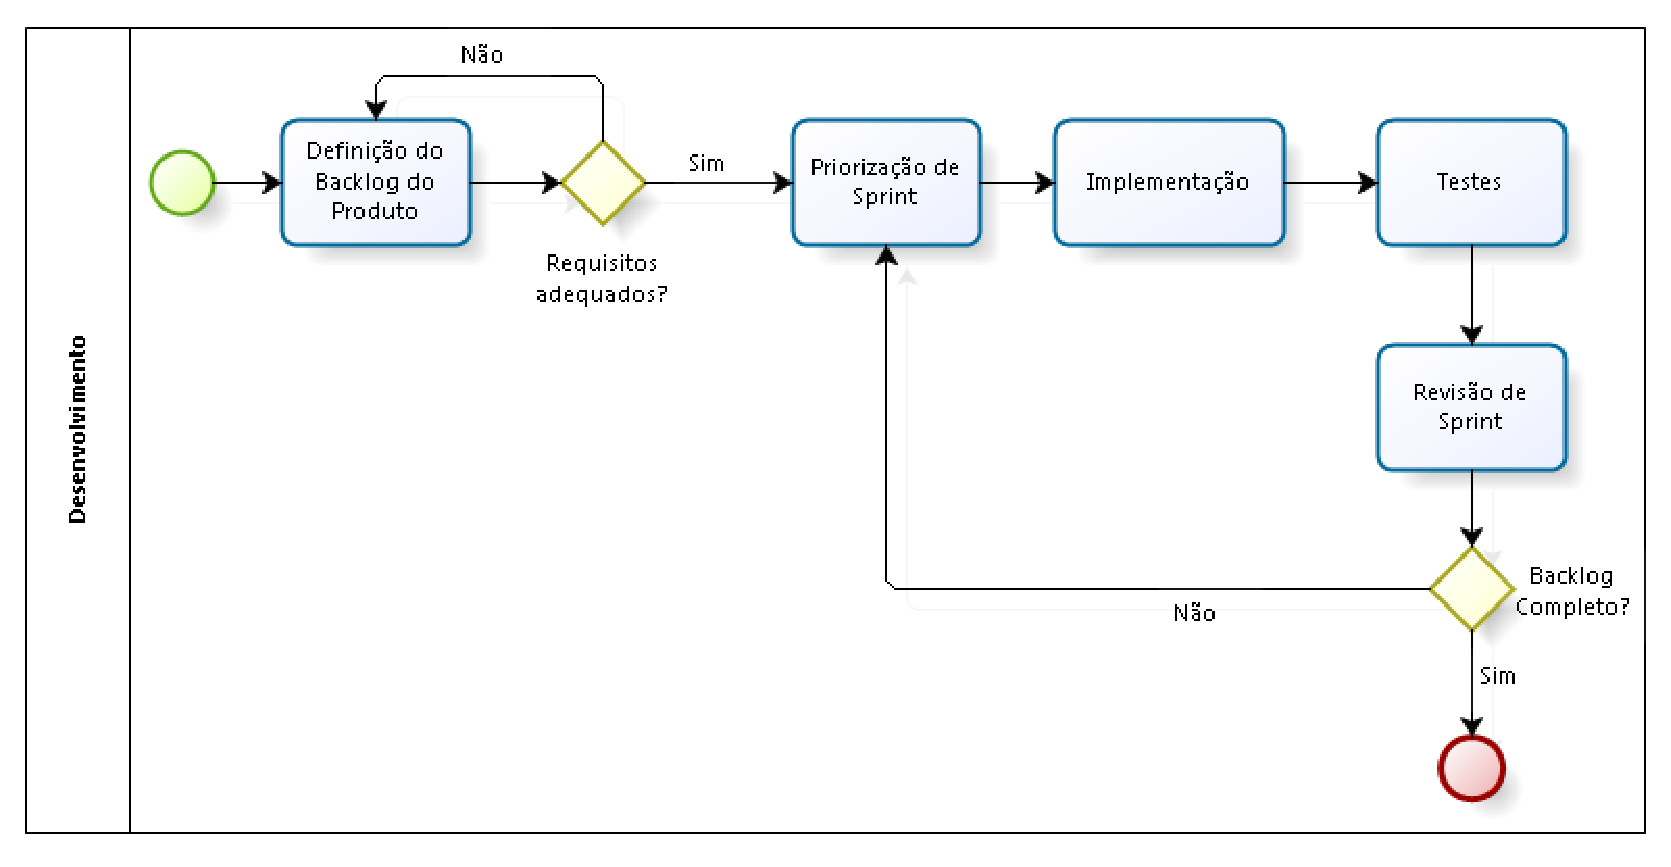
\includegraphics[scale=0.4]{figuras/capitulo4/processo_desenvolvimento.eps}
	\caption{Processo de desenvolvimento}
	\label{Processo desenvolvimento}
\end{figure}

Ao se observar a Figura \ref{Processo desenvolvimento}, teve-se a etapa inicial de criação do \textit{backlog} do produto. Quando completo, deu-se inicio a um fluxo de desenvolvimento que passou por etapas de desenvolvimento e testes em \textit{sprints}.

\section{Cronograma}

A seguir, nas Figuras \ref{cronograma_parte_1} e \ref{cronograma_parte_2}, são apresentados os cronogramas preliminares referentes às atividades que foram realizadas durante todo este trabalho. Estes cronogramas estão divididos entre as atividades das etapas um (que abrange o período entre agosto de 2015 e dezembro de 2015) e dois (que abrange o período entre março e julho de 2016).

\begin{figure}[h]
	\centering
	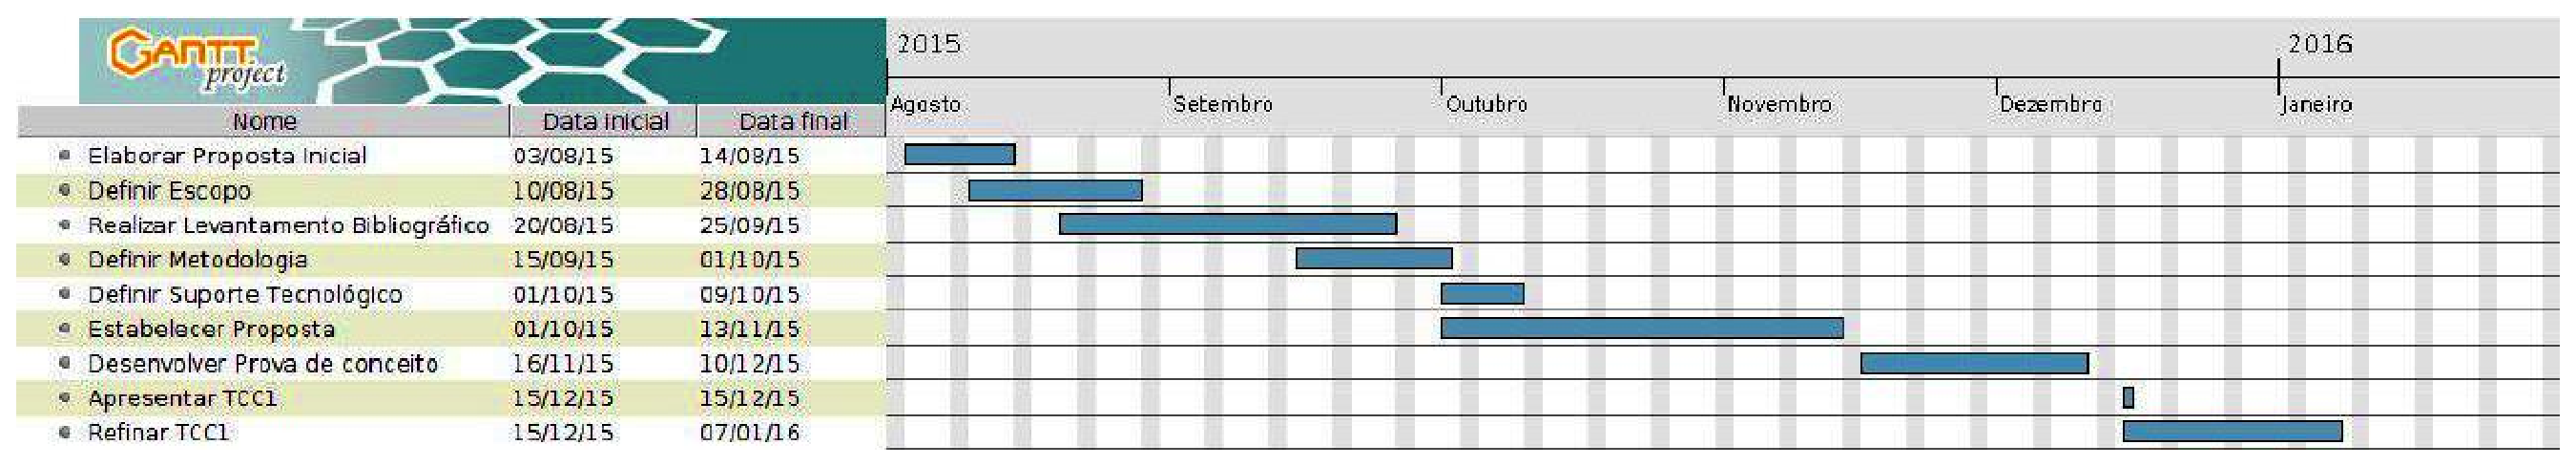
\includegraphics[scale=0.4]{figuras/capitulo4/gant1.eps}
	\caption{Cronograma primeira parte}
	\label{cronograma_parte_1}
\end{figure}

\begin{figure}[h]
	\centering
	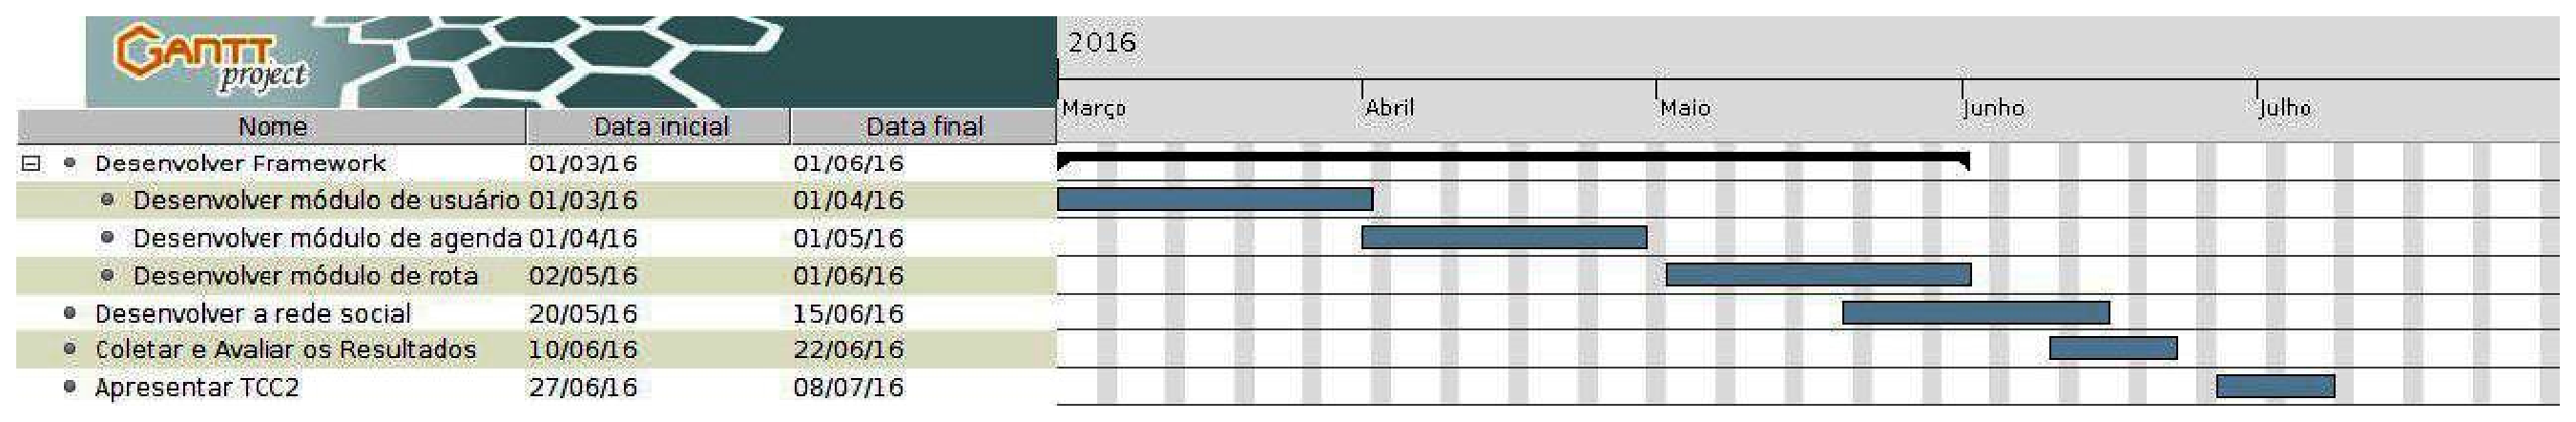
\includegraphics[scale=0.4]{figuras/capitulo4/gant2.eps}
	\caption{Cronograma segunda parte}
	\label{cronograma_parte_2}
\end{figure}

\section{Resumo do Capítulo}

Este capítulo apresentou as metodologias que foram utilizadas durante a realização das pesquisas e do desenvolvimento deste trabalho.

Inicialmente, foram documentadas, no apêndice, diversas metodologias. Essas metodologias estão divididas de acordo com o ponto de vista da natureza da pesquisa, da forma de abordagem, dos objetivos e dos procedimentos técnicos. Com a apresentação dessas metodologias, foram selecionadas as que melhor se adequavam a este trabalho. A metodologia de desenvolvimento seguiu práticas ágeis e está baseada no Scrum.

Foi apresentado também o fluxo de trabalho com as atividades definidas para as duas etapas de desenvolvimento deste trabalho bem como o cronograma proposto para cumprimento destas atividades.

O próximo capítulo apresentará a proposta consolidada, a qual orientou o processo de desenvolvimento desse trabalho.
